% !TEX root = perelman-geometry.tex
%!TEX TS-program = pdflatex
%!TEX encoding = UTF-8 Unicode


%\maketitle
\cleardoublepage
\thispagestyle{empty}
%\pagenumbering{roman}
\begin{fullwidth}
\begin{center}

{\LARGE \emph{Ya. I. Perelman}}

{\Huge Geometry\\ for \\ Entertainment}\\[2cm]




The Mir Titles Project\\

{\small Translated from the Russian by \emph{Damitr Mazanav}}

\end{center}
\end{fullwidth}
\cleardoublepage

\thispagestyle{empty}
\vfill
\begin{small}

{\noindent

Translated from the Russian and typeset in \LaTeX{} using Linux Libertine by \emph{Damitr Mazanav} from the Seventh revised edition published in 1950.


This fully electronic English translation released in 2024 by \\\textsc{the mir titles project} \url{https://mirtitles.org} .

\href{https://gitlab.com/mirtitles/perelman-geometry}{Link} to the source files. 
 
Front cover: Woodcut from Cosimo Bartoli's \href{https://archive.org/details/cosimobartolidel00bart}{\emph{Del modo di misvrare}} published in 1564. 

\copyright \emph{Damitr Mazanav} \href{mailto:damitr@proton.me}{damitr@proton.me}

Licence Creative Commons by NC Sharealike 4.0


\includegraphics[width=0.3\textwidth]{figures/Cc-by-nc-sa_icon.pdf}

Перельман Я.И. Занимательная геометрия. Москва-Ленинград: Государственное издательство технико-теоретической литературы, 1950

\href{https://archive.org/details/20220910_perelman_geometry/}{Original} Seventh revised edition in Russian published in 1950 by  \emph{State Publishing House Of Technical And Theoretical Literature}, Moscow -- Leningrad.

Edited and supplemented by \emph{B.A. Kordemsky}
}

\end{small}

\cleardoublepage
\thispagestyle{empty}
\vspace*{\fill}
\begin{center}
\textsc{\large about mir titles project}
\end{center}
\marginnote{
\url{https://mirtitles.org}
\url{https://archive.org/details/mir-titles}}
The Mir Titles project aims to preserve the wealth of knowledge encapsulated in various books published during the Soviet era for future generations. This extensive collection features works on science, mathematics, philosophy, popular science, and history, as well as large number of books on Soviet, Russian, and children's literature in several languages. The project has been made possible through the generous support and contributions from friends and supporters worldwide.






 
 \cleardoublepage

\chapter{Editor's Preface}
\label{editor-preface}
%\addcontentsline{toc}{chapter}{\nameref{preface}}


\emph{Geometry for Entertainment} is written both for friends of mathematics and for those readers from whom many attractive aspects of mathematics have somehow been hidden.

More importantly, this book is intended for those readers who studied (or are currently studying) geometry only at the blackboard and therefore are not used to noticing familiar geometric relationships in the world of things and phenomena around us, have not learnt to use the acquired geometric knowledge in practise, in difficult cases of life, on a hike, in a bivouac or front-line situation.

To arouse the reader's interest in geometry or, in the words of the author, ``to inspire a desire and cultivate a taste for its study is the objective of this book.''

To this end, the author will take geometry ``out of the walls of the school room into the free air, into the forest, field, to the river, on the road, in order to indulge in relaxed geometric studies without a textbook and tables in the open air \ldots{}'', and draws the reader's attention to the pages of L. N. Tolstoy and A. P. Chekhov, Jules Verne and Mark Twain. He finds a theme for geometric problems in the works of N. V. Gogol and A. S. Pushkin, and finally offers the reader ``a motley selection of problems, curious in plot, unexpected in result.''

The seventh edition of \emph{Geometry for Entertainment} is published without the direct participation of the author. Ya. I. Perelman died in Leningrad in 1942.

The new edition of the book contains almost all the articles of the previous edition, newly illustrated, edited and supplemented with facts and information from our Soviet reality, as well as a considerable number (about 30) additional articles.

I was guided by the desire to increase the ``utility coefficient'' of Ya. Perelman's book, to make it even more effective and interesting, involving new readers in the ranks of friends of mathematics.

To what extent this was possible, I hope to learn from readers at the address: Moscow, 64, Chernyshevsky Str., 81, Sq. 53, B. A. Kordemsky.


\begin{flushright}
\emph{B. Kordemsky}
\end{flushright}


\chapter{Translator's Preface}
\label{translator-preface}
%\addcontentsline{toc}{chapter}{\nameref{preface}}


Yakov Perelman's books have been a constant source of inspiration for me throughout my life. Though many of his works have been translated into English and other languages, several remain untranslated. As the overarching aim of the Mir Titles Project, we endeavour to bring all such works to the public. This translation was a rather ambitious project, and I was not sure of the time it would require. But the project got completed in little over a months time. It brings me great pleasure to present this English translation of untranslated work of Perelman.


\marginnote{Examples}Perelman, in his discussions, emphasises the geometrical relationships in measurable and unknown quantities. This approach is historical in the sense that this is how geometry developed: to solve problems of measurement of unknown quantities. 

The book has two sections, the first one, \emph{Geometry In The Open Air} is oriented towards the ``field'' aspect, involving measurements of variety of things, using direct and indirect measurements using very basic instruments, including our body parts. 


The second part of the book, \emph{Between Seriousness And Joke In Geometry}, delves into more whimsical and application aspects of geometry. Many discussions are based on legends and literature in which Perelman investigates geometrical aspects of the situations depicted. A lot of the content of the book focuses on practical aspects of applying geometry to solve problems that we might face in open fields, by the river, in the sky, in the ocean, during constructions, in scaling objects for measuring angles, lengths, areas, and volumes, among other things. I am sure that after reading this book, you will see mathematics embedded in many familiar objects. 


\marginnote{Illustrations}The beautiful and abundant illustrations are the heart of the book. Geometry, being primarily reliant on graphics, is brought to life in a variety of situations. Familiar geometrical shapes, lines, and ratios are found among trees, rivers, homes, skies, and other natural settings. 

Each topic is complemented by relevant illustrations, which makes visualising and understanding them easier. I have made no effort to change the images, except in some cases where I replaced the Russian words with English ones. Only one image had to be completely redrawn, as the original was not of good quality.

\marginnote{Translation}I have made use of machine translations for the bulk of the text, and the results are quite satisfactory. At times, I have used several translation services to ensure I am on the right track and that the meaning is not lost in translation. Though, of course, there might be places where I have not translated correctly. I learnt to read the Russian in a very rudimentary way in the process. :)

At places I have added my own notes for clarification which are indicated by my initials at the end -- \textsc{dm}.

\marginnote{Typesetting}
I have typeset the book in a square profile with marginpar for figures and notes. This design helps in making the book more readable by trying to keep the figures and notes on the same page. During the course of typesetting this book, several challenges in \LaTeX{} were resolved by the discussions and questions posted on \href{https://tex.stackexchange.com}{tex.stackexchange}. I am really grateful to the experts in the forum whose answers helped me learn a lot and resolve the typographical and technical challenges.

If there are any mistakes in the mathematics or translation, they are all mine. Any suggestions and criticisms to improve the translation and the design of the book are welcome.\marginnote{Please drop your suggestions  on the Mir Titles blog or write to \href{mailto:mirtitles@gmail.com}{mirtitles@gmail.com}} Translating this book was a great learning experience for me in several ways. I hope that this English version finds enthusiastic readers and inspires many more brilliant minds in the generations to come.


\begin{flushright}
\emph{Damitr Mazanav}\\
\textsc{mumbai, may 2024}\\[10pt]
%\begin{figure}[!h]
%\centering
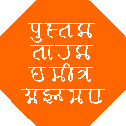
\includegraphics[width=0.25\textwidth]{figures/pustaktarak.pdf}
%\end{figure}
\end{flushright}

\clearpage